\documentclass{article}

\usepackage{amsmath} % For mathematical symbols and environments
\usepackage{amssymb} % For additional mathematical symbols
\usepackage{tcolorbox}
\usepackage{pgfplots}

\newtcolorbox{esbox}{
    colback=blue!5!white,
    colframe=blue!75!black,
    fonttitle=\bfseries,
    title=Esempio
}

\title{Definizioni}
\author{Agostino Cesarano}
\date{January 2024}

\begin{document}

\maketitle

\section*{Premesse}
%Intorno%
Si definisce intorno di ampiezza $\varepsilon$ e centro $l$ l'insieme
$I_\varepsilon(l) = \{x\in\mathbb{R}:|x-l|<\varepsilon\}$.
\[I_\varepsilon(l) = (l-\varepsilon,l+\varepsilon)\]
\[
    \begin{tikzpicture}
        \draw[latex-latex] (-3,0) -- (3,0) ; % draws 1-d number line
        \draw[shift={(-1,0)},color=black] (0pt,0pt) -- (0pt,-9pt) node[below]
        {$l-\varepsilon$}; % draws ticks
        \draw[shift={(1,0)},color=black] (0pt,0pt) -- (0pt,-9pt) node[below]
        {$l+\varepsilon$}; % draws ticks
        \draw[very thick,red] (-1,0) -- (1,0); % interval for epsilon neighborhood
        \draw[shift={(0,0)},color=black] (0pt,0pt) -- (0pt,9pt) node[above]
        {$l$}; % point x
        \node at (0,0) {$\bullet$}; % point x
    \end{tikzpicture}
\]
%Punto di accumulazione%
Si dice che $l$ è un punto di accumulazione di $A\subseteq\mathbb{R}$ se ogni
intorno di $l$ contiene almeno un punto di $A$ diverso da $l$.
\[
    \begin{tikzpicture}
        \draw[latex-latex] (-3,0) -- (3,0) ; % draws 1-d number line
        \draw[shift={(-1,0)},color=black] (0pt,0pt) -- (0pt,-9pt) node[below]
        {$l-\varepsilon \in A$}; % draws ticks
        \draw[shift={(1,0)},color=black] (0pt,0pt) -- (0pt,-9pt) node[below]
        {$l+\varepsilon$}; % draws ticks
        \draw[very thick,red] (-1,0) -- (1,0); % interval for epsilon neighborhood
        \draw[shift={(0,0)},color=black] (0pt,0pt) -- (0pt,9pt) node[above]
        {$l$}; % point x
        \node at (0,0) {$\bullet$}; % point x
    \end{tikzpicture}
\]
In un intorno di un punto di accumulazione di $A$ ci sono infiniti punti di
$A$.
%Punto isolato%
Si dice che $l$ è un punto isolato di $A\subseteq\mathbb{R}$ se $l\in A$ e $l$
non è un punto di accumulazione di $A$. Quindi, se $l$ è un punto isolato di
$A$, allora $\exists\varepsilon>0$ tale che $I_\varepsilon(l)\cap A=\{l\}$.
\[
    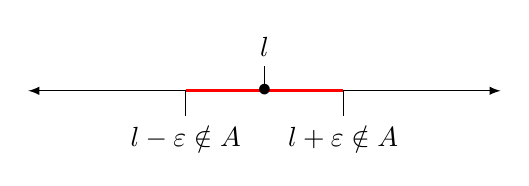
\begin{tikzpicture}
        \draw[latex-latex] (-3,0) -- (3,0) ; % draws 1-d number line
        \draw[shift={(-1,0)},color=black] (0pt,0pt) -- (0pt,-9pt) node[below]
        {$l-\varepsilon \notin A$}; % draws ticks
        \draw[shift={(1,0)},color=black] (0pt,0pt) -- (0pt,-9pt) node[below]
        {$l+\varepsilon \notin A$}; % draws ticks
        \draw[very thick,red] (-1,0) -- (1,0); % interval for epsilon neighborhood
        \draw[shift={(0,0)},color=black] (0pt,0pt) -- (0pt,9pt) node[above]
        {$l$}; % point x
        \node at (0,0) {$\bullet$}; % point x
    \end{tikzpicture}
\]
%Intorno bucato%
Si dice che $l$ è un punto di accumulazione bucato di $A\subseteq\mathbb{R}$ se
$l$ è un punto di accumulazione di $A$ ma non è un punto di $A$.\\\\
\[
    \begin{tikzpicture}
        \draw[latex-latex] (-3,0) -- (3,0) ; % draws 1-d number line
        \draw[shift={(-1,0)},color=black] (0pt,0pt) -- (0pt,-9pt) node[below]
        {$l-\varepsilon \in A$}; % draws ticks
        \draw[shift={(1,0)},color=black] (0pt,0pt) -- (0pt,-9pt) node[below]
        {$l+\varepsilon$}; % draws ticks
        \draw[very thick,red] (-1,0) -- (1,0); % interval for epsilon neighborhood
        \draw[shift={(0,0)},color=black] (0pt,0pt) -- (0pt,9pt) node[above]
        {$l$}; % point x
        \node at (0,0) {$\times$}; % point x
    \end{tikzpicture}
\]
\setcounter{part}{1}
\part{Limiti}
Sia $f:A\subseteq\mathbb{R}\rightarrow\mathbb{R}$ una funzione e sia $l$ un
punto di accumulazione di $A$. Si dice che $l$ è il limite di $f(x)$ per $x$
che tende a $l$ se $\forall\varepsilon>0$ esiste $\delta>0$ tale che
$0<|x-l|<\delta\Rightarrow|f(x)-l|<\varepsilon$.
\begin{equation}
    \begin{cases}
        (x - l) < \delta \\
        -(x - l) < \delta
    \end{cases}
\end{equation}

\[ l - \delta < x < l + \delta\]
\[
    \Rightarrow
\]

\begin{equation}
    \begin{cases}
        f(x) - l < \varepsilon \\
        -(f(x) + l) < \varepsilon
    \end{cases}
\end{equation}

\[l-\varepsilon < f(x) < l + \varepsilon\]

Quindi preso un $\delta$ qualsiasi tale che $x$ è compreso tra $l-\varepsilon$
e $l+\varepsilon$, esiste un $\varepsilon$ tale che $f(x)$ è compreso tra
$l-\varepsilon$ e $l+\varepsilon$.
%Relazione tra limiti di funzioni e limiti di successioni%
\section*{Relazione tra limiti di funzioni e limiti di successioni}
Le proprietà di convergenza di una successione $a_n$ sono le stesse di una funzione $f(x)$.
%Alcuni limiti notevoli%
\section*{Limiti notevoli}
% Nuovca numerazione delle equazioni%
\setcounter{equation}{0}
\begin{equation}
    \lim_{x\to+\infty}a^x=
    \begin{cases}
        0       & 0<a<1 \\
        +\infty & a>1   \\
    \end{cases}
\end{equation}
\begin{equation}
    \lim_{x\to-\infty}a^x=
    \begin{cases}
        +\infty & 0<a<1 \\
        0       & a>1   \\
    \end{cases}
\end{equation}
\begin{equation}
    \lim_{x\to+\infty}x^b=
    \begin{cases}
        0       & b<0 \\
        +\infty & b>0 \\
    \end{cases}
\end{equation}
\begin{equation}
    \lim_{x\to+\infty}e^x=+\infty
\end{equation}
\begin{equation}
    \lim_{x\to-\infty}e^x=\lim_{x\to+\infty}\frac{1}{e^x}=0
\end{equation}
\begin{equation}
    \lim_{x\to+\infty}\frac{e^x-1}{x}=1
\end{equation}
\begin{equation}
    \lim_{x\to+\infty}\log x=+\infty
\end{equation}
\begin{equation}
    \lim_{x\to0^+}\log x=-\infty
\end{equation}
\begin{equation}
    \lim_{x\to-\infty}\log x \quad\text{non esiste}
\end{equation}
\begin{equation}
    \lim_{x\to+\infty}x^b \log x =0
\end{equation}
\begin{center}
    Gerarchia degli infiniti in ordine crescente:
    \[\log x, \quad x^b, \quad a^x, \quad x!, \quad x^x \]
    Valgono quindi i sequenti limiti notevoli:
\end{center}
\begin{equation}
    \lim_{x\to+\infty}\frac{\log x}{x^b}=0 \quad (b>0)
\end{equation}
\begin{equation}
    \lim_{x\to+\infty}\frac{x^b}{a^x}=0 \quad (a>1,b>0)
\end{equation}
\begin{equation}
    \lim_{x\to+\infty}\frac{a^x}{x!}=0
\end{equation}
\begin{center}
    Molto importante è il seguente limite notevole:
\end{center}
\begin{equation}
    \lim_{x\to+\infty}\left(1+\frac{1}{x}\right)^x=e
\end{equation}
\begin{equation}
    \lim_{x\to-\infty}\left(1+\frac{1}{x}\right)^x=e
\end{equation}
\begin{center}
    Limiti notevoli per le successioni trigonometriche:
\end{center}
\begin{equation}
    \lim_{x\to\pm\infty}\sin x \quad\text{non esiste}
\end{equation}
\begin{equation}
    \lim_{x\to\pm\infty}\cos x \quad\text{non esiste}
\end{equation}
\begin{equation}
    \lim_{x\to\pm\infty}\tan x \quad\text{non esiste}
\end{equation}
\begin{equation}
    \lim_{x\to+\infty}\arctan x=\frac{\pi}{2}
\end{equation}
\begin{equation}
    \lim_{x\to-\infty}\arcsin x=-\frac{\pi}{2}
\end{equation}
\begin{equation}
    \lim_{x\to0}\frac{\sin x}{x}=1
\end{equation}
\begin{equation}
    \lim_{x\to0}\frac{1-\cos x}{x^2}=\frac{1}{2}
\end{equation}

\end{document}